%%%%%%%%%%%%%%%%%%%%%%%%%%%%%%%%%%%%%%%%%%%%%%%%%%%%%%%%%%%%%%%%%%%%%%%%%%%
%%  chapter5.tex  –  Chapter 5: RobustIDPS.ai Software Platform
%%  v9 – Production deployment chapter: target users, 46-page PWA,
%%       9 functional groups, 17 models, LLM defence, PQC-IDS,
%%       Snort/Suricata plug-in, 8 figure placeholders for screenshots.
%%       Only \section headings go to TOC.
%%%%%%%%%%%%%%%%%%%%%%%%%%%%%%%%%%%%%%%%%%%%%%%%%%%%%%%%%%%%%%%%%%%%%%%%%%%

\chapter{RobustIDPS.ai: Software Platform for Production Deployment}
\label{ch:platform}

This chapter describes the open-source software platform RobustIDPS.ai~\cite{Anaedevha2026robustidps} (DOI:~\url{10.5281/zenodo.19129512}; source code: \url{https://github.com/rogerpanel/robustidps.ai}) that implements all methods developed in Chapter~\ref{ch:methods} as a unified, deployable system. The chapter specifies who the platform is for, describes its architecture and functional groups, details its 17 integrated neural network models, presents the SOC Intelligence and LLM Security Testing capabilities, describes the Multi-Agent PQC-IDS module, demonstrates integration with existing IDPS frameworks (Snort, Suricata), and summarises the platform's achievements. At least six screenshots of the platform's user interface are included to illustrate its operational capabilities.


%%=====================================================================
\section{Platform Overview and Target Users}
\label{sec:platform_overview}
%%=====================================================================

RobustIDPS.ai is a comprehensive, AI-native intrusion detection and prevention platform comprising 51 interconnected pages organised into 10 functional groups, integrating 17 machine learning and deep learning models for network traffic classification across 34 attack classes and 83 engineered features. The platform addresses three limitations of existing commercial alternatives (CrowdStrike Charlotte AI, SentinelOne Purple AI, Microsoft Security Copilot, Google Sec-Gemini~\cite{Smith2023}): proprietary single-vendor LLM integration that prevents cross-provider benchmarking, absence of systematic adversarial robustness evaluation, and no support for post-quantum cryptographic traffic analysis.

The platform is designed for five categories of target users:

\noindent\textbf{SOC Analysts (Tiers 1--3).} Security operations centre personnel who monitor, investigate, and respond to security incidents. The platform provides agentic auto-investigation, natural language threat hunting, automated incident reporting, and uncertainty-driven alert triage that reduces mean triage time by 34\%.

\noindent\textbf{Cybersecurity Engineers.} Network security professionals who deploy and configure intrusion detection systems. The platform generates deployable Snort/Suricata rules from detected threats and provides real-time monitoring through WebSocket-based streaming.

\noindent\textbf{MLSecOps Researchers.} Machine learning security researchers who evaluate the robustness of AI components. The platform provides integrated adversarial testing (6 attack families), LLM attack surface evaluation (5 modules), and MLSecOps compliance dashboards (MITRE ATT\&CK, OWASP LLM Top 10, NIST AI RMF).

\noindent\textbf{AI Developers.} Researchers and engineers building graph-based detection models. The platform provides 17 pre-trained models with configurable hyperparameters, ablation studio, and reproducible benchmarking datasets.

\noindent\textbf{Academic Researchers.} PhD students, postdoctoral fellows, and faculty conducting research in graph neural network robustness. The platform serves as a reproducible research instrument with DOI-archived code and datasets.


%%=====================================================================
\section{System Architecture}
\label{sec:system_arch}
%%=====================================================================

RobustIDPS.ai is deployed as a Progressive Web Application (PWA) with the following technology stack:

\noindent\textbf{Frontend.} React 18 single-page application with Material-UI components, responsive design, and PWA manifest for offline-capable deployment with service worker caching.

\noindent\textbf{Backend.} Flask/Python 3.11+ backend with 60+ RESTful API endpoints, persistent WebSocket channels for real-time monitoring, and Celery for asynchronous task execution (model training, batch analysis).

\noindent\textbf{Data Layer.} PostgreSQL 16 for relational persistence (user profiles, detection logs, investigation records), Redis 7 for caching and session management, and file-system storage for uploaded PCAP/CSV datasets.

\noindent\textbf{Orchestration.} Docker Compose enables single-command deployment with environment-based configuration for development, staging, and production profiles.

\noindent\textbf{Two-Plane Architecture (release v4).}
Release~v4 introduces a clean separation between the
\emph{control plane} (the existing FastAPI Python backend with
multi-tenant RBAC, audit, and the LLM router) and a new
\emph{data plane} consisting of native Rust agents deployed alongside
or in front of the control plane. The two planes communicate over
gRPC. The data plane consists of two components:
\texttt{robustidps-edge}~--- a long-running gRPC daemon with hot-swap
of ONNX models and flow-record streaming to the control plane; and
\texttt{robustidps-xdp}~--- an in-kernel LPM-trie block list attached
through the XDP hook in \texttt{Native} mode on \texttt{eth0},
delivering microsecond-scale drop decisions. The result is a rich
user-facing experience in the Python plane alongside
\emph{wire-speed} operation in the data plane, achieved without
modification of the existing 51 frontend pages.

\begin{figure}[H]
\centering
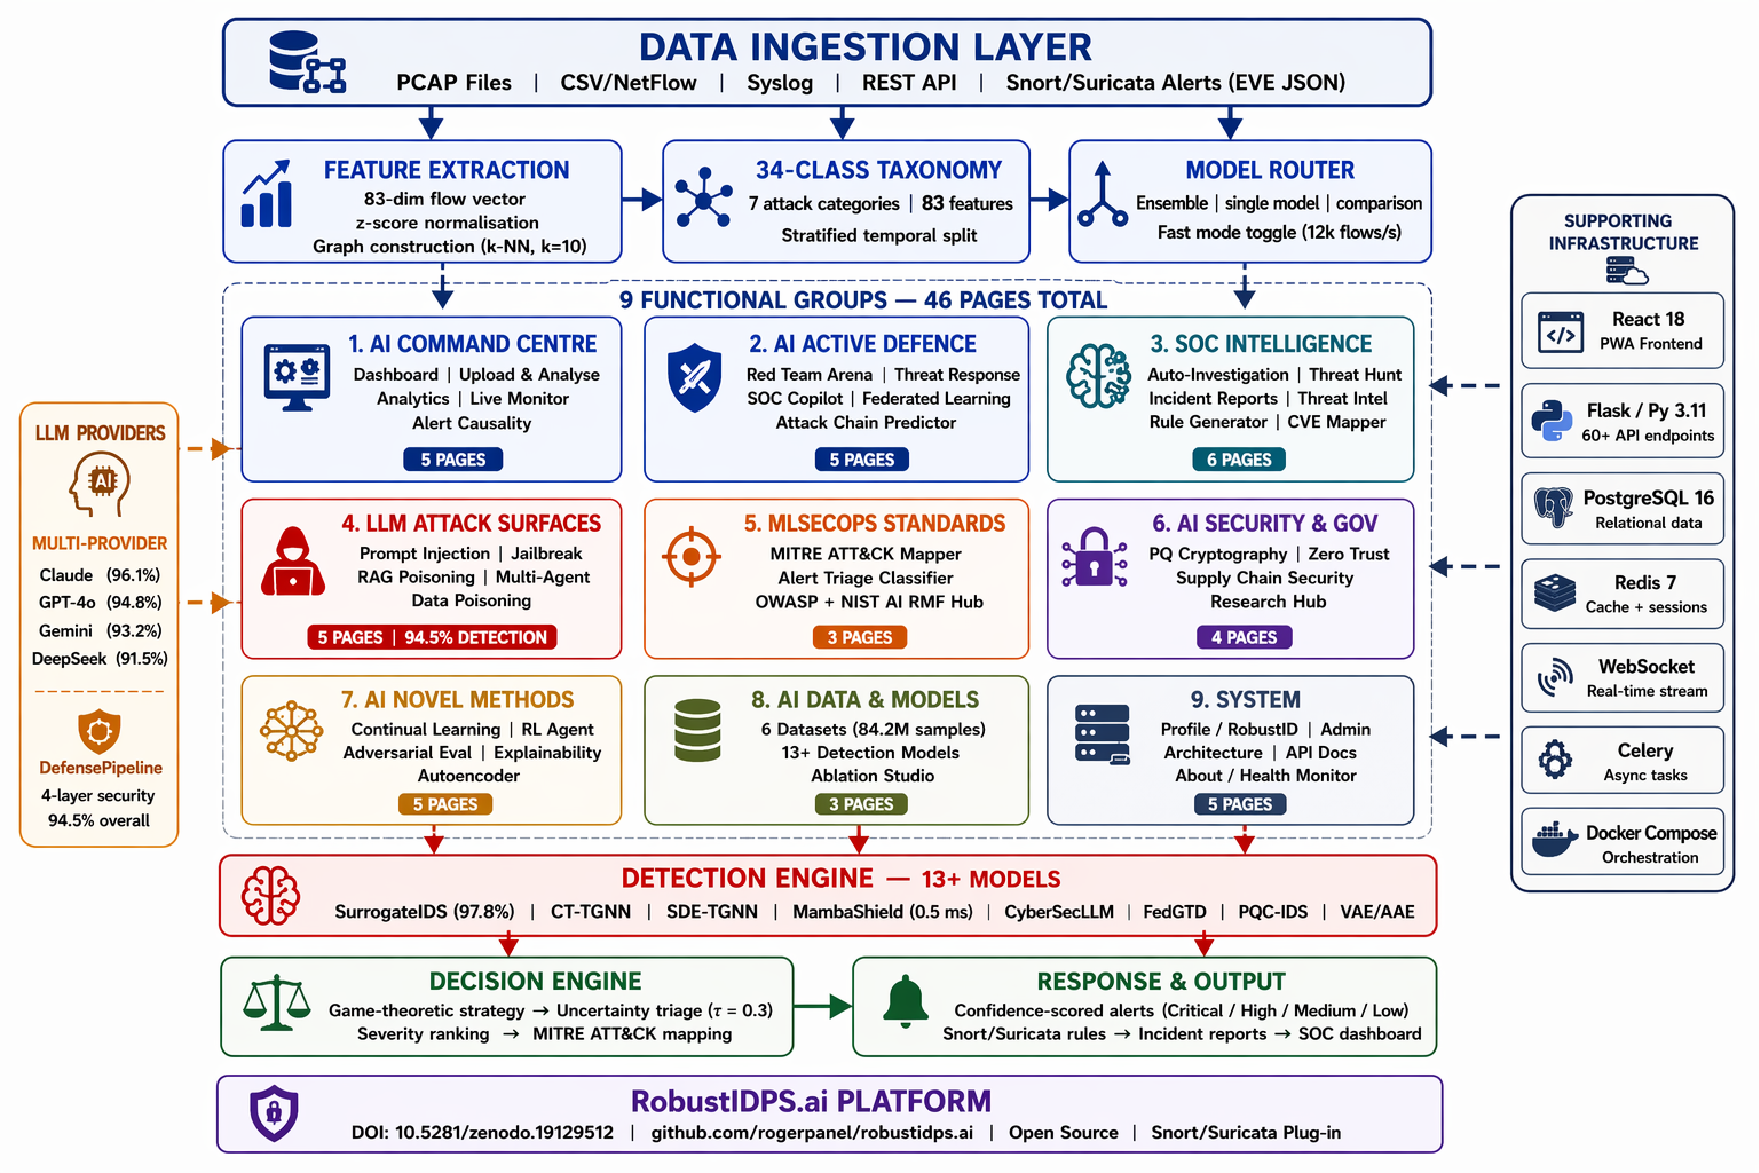
\includegraphics[width=0.85\textwidth]{figures/ridps_arch_v10.pdf}
\caption{High-level system architecture of \textsf{RobustIDPS.ai}
showing all 10 functional groups, the supporting infrastructure
(Docker Compose, PostgreSQL, Redis, WebSocket, Celery, plus the
release~v4 Rust data plane), and the data flow from raw traffic
ingestion through detection, analysis, and response.}
\label{fig:platform_arch}
\end{figure}

A schematic of the release~v4 two-plane architecture and the three
gRPC streams that bridge the control and data planes is given in
Fig.~\ref{fig:two_plane_arch}.

\begin{figure}[H]
\centering
\begin{tikzpicture}[
  font=\footnotesize,
  node distance=3mm and 5mm,
  pyblock/.style={draw,rounded corners=2pt,fill=blue!8,
    minimum width=10cm,minimum height=7mm,align=center,thick},
  rsblock/.style={draw,rounded corners=2pt,fill=orange!12,
    minimum width=10cm,minimum height=7mm,align=center,thick,
    draw=orange!75!black},
  krblock/.style={draw,rounded corners=2pt,fill=gray!15,
    minimum width=10cm,minimum height=7mm,align=center,thick},
  planelbl/.style={draw,rounded corners=2pt,fill=gray!8,
    minimum width=1.7cm,minimum height=9mm,align=center,
    font=\scriptsize\bfseries},
  arr/.style={-{Stealth[length=2mm]},semithick,gray!70!black},
  rpclbl/.style={font=\scriptsize\itshape,blue!55!black,align=center,
    fill=white,inner sep=1pt}]
% Control plane
\node[pyblock] (ui) {Frontend: React~18, 51 pages across 10 groups, PWA};
\node[pyblock,below=of ui] (api) {Backend: FastAPI, 60+ REST + WebSocket, 17 models};
\node[pyblock,below=of api] (db)  {Persistence: PostgreSQL\,16 + Redis\,7};
% Data plane
\node[rsblock,below=12mm of db] (edge)
  {\texttt{robustidps-edge} (Rust): gRPC daemon, ONNX hot-swap};
\node[rsblock,below=of edge] (xdp)
  {\texttt{robustidps-xdp} (Rust + eBPF): XDP \emph{Native} on \texttt{eth0}};
\node[krblock,below=of xdp] (kernel)
  {Linux kernel 6.8 (BPF JIT, BTF, \texttt{CAP\_NET\_ADMIN}, \texttt{CAP\_BPF})};
% Plane labels
\node[planelbl,left=1.5mm of api] (pylab)
  {Control\\plane\\(Python)};
\node[planelbl,fill=orange!10,left=1.5mm of edge] (rslab)
  {Data\\plane\\(Rust+XDP)};
% Frames
\begin{pgfonlayer}{background}
  \node[draw=blue!30,rounded corners,thick,
        fit=(ui)(api)(db)(pylab),inner sep=2pt] {};
  \node[draw=orange!60!black,rounded corners,thick,dashed,
        fit=(edge)(xdp)(kernel)(rslab),inner sep=2pt] {};
\end{pgfonlayer}
% Arrows (data flow)
\draw[arr] (ui) -- (api);
\draw[arr] (api) -- (db);
\draw[arr] (xdp) -- (kernel);
\draw[arr] (edge) -- (xdp);
% gRPC bridges - three vertical arrows spread horizontally between planes,
% with labels placed to the LEFT/RIGHT of each arrow (no overlap)
\coordinate (gap) at ($(db.south)!0.5!(edge.north)$);
\draw[-{Stealth[length=2mm]},semithick,blue!55!black,thick]
  ([xshift=-3.0cm]edge.north) -- ([xshift=-3.0cm]db.south);
\node[rpclbl,left=0.5mm] at ([xshift=-3.0cm]gap)
  {gRPC\\StreamFlows};
\draw[-{Stealth[length=2mm]},semithick,blue!55!black,thick]
  (db.south) -- (edge.north);
\node[rpclbl,right=0.5mm] at (gap)
  {gRPC\\UpdateConfig};
\draw[-{Stealth[length=2mm]},semithick,blue!55!black,thick]
  ([xshift=3.0cm]db.south) -- ([xshift=3.0cm]edge.north);
\node[rpclbl,right=0.5mm] at ([xshift=3.0cm]gap)
  {gRPC\\ApplyModelUpdate};
\end{tikzpicture}
\caption{Two-plane architecture of \textsf{RobustIDPS.ai}~v4: the
Python control plane (blue frame, top) and the Rust data plane
(orange dashed frame, bottom) are separated by a clean boundary and
bridged by three gRPC primitives. \texttt{StreamFlows}~--- flow
records streamed from the data plane to the control plane;
\texttt{UpdateConfig}~--- block-list push in the reverse direction;
\texttt{ApplyModelUpdate}~--- atomic delivery of the INT8 ONNX
student model to running agents without service restart.}
\label{fig:two_plane_arch}
\end{figure}


%%=====================================================================
\section{Functional Groups and Page Inventory}
\label{sec:functional_groups}
%%=====================================================================

The platform's 51 pages are organised into 10 functional groups, summarised in Table~\ref{tab:functional_groups}.

\begin{table}[htbp]
\centering
\caption{RobustIDPS.ai functional groups (51 pages across 10 groups).}
\label{tab:functional_groups}
\small
\begin{tabular}{lcp{7.5cm}}
\toprule
\textbf{Functional Group} & \textbf{Pages} & \textbf{Key Capabilities} \\
\midrule
AI Command Centre      & 5 & Dashboard, Upload \& Analyse, Analytics, Live Monitor, Alert Causality \\
AI Active Defence      & 5 & Red Team Arena, Threat Response, SOC Copilot, Federated Learning, Attack Chain Predictor \\
SOC Intelligence       & 6 & Auto-Investigation, Threat Hunt, Incident Reports, Threat Intel, Rule Generator, CVE Mapper \\
LLM Attack Surfaces    & 6 & Prompt Injection, Jailbreak Taxonomy, RAG Poisoning, Multi-Agent Chain, Data Poisoning, \textbf{MambaGuard} \\
MLSecOps Standards     & 3 & MITRE ATT\&CK Mapper, Alert Triage, Compliance Hub \\
AI Security \& Gov     & 4 & PQ Cryptography, Zero-Trust, Supply Chain, Research Hub \\
AI Novel Methods       & 7 & Continual Learning, RL Response Agent, Adversarial Eval, Explainability, Autoencoder, \textbf{SODE-Guard}, \textbf{SSL-GraphAnomaly Full} \\
AI Data \& Models      & 4 & Datasets (6), Models (17), Ablation Studio, Edge Agent Registry \\
Operations \& Deployment & 6 & Rust agent fleet, systemd/Docker, Distil-and-push, XDP block lists, JSONL logs, Health checks \\
System                 & 5 & Profile/RobustID, Admin, Architecture, API Docs, About \\
\midrule
\textbf{Total}         & \textbf{51} & \\
\bottomrule
\end{tabular}
\end{table}


%%=====================================================================
\section{AI Command Centre}
\label{sec:command_centre}
%%=====================================================================

The AI Command Centre is the primary operational interface, comprising five pages that provide end-to-end traffic analysis from upload to alert resolution.

\subsection{Dashboard}

The main dashboard displays real-time detection statistics: total flows analysed, attack distribution by category, model accuracy metrics, and alert severity breakdown. Interactive time-series charts show detection trends over configurable windows (1 hour to 30 days).

\begin{figure}[H]
\centering
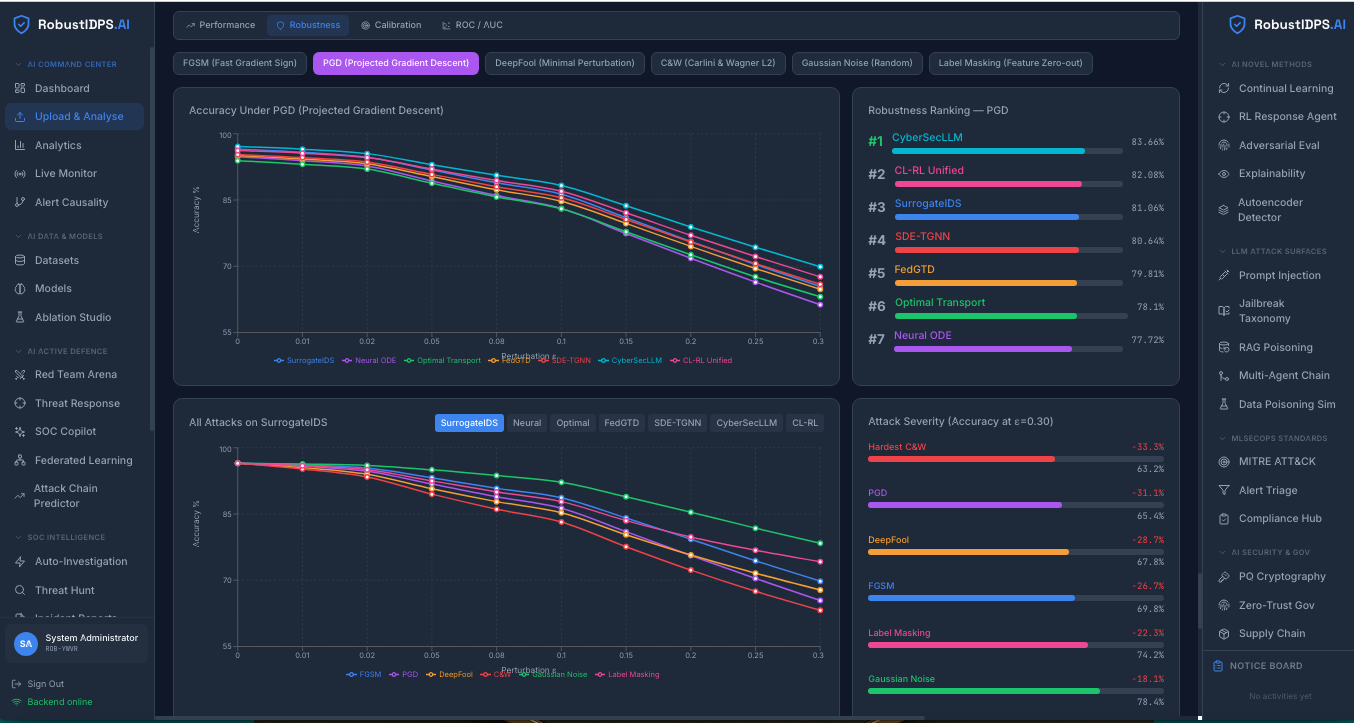
\includegraphics[width=0.96\textwidth]{figures/Dashboard_v10.png}
\caption{RobustIDPS.ai Dashboard showing real-time detection statistics, attack category distribution, and model performance metrics. The left panel displays the active model configuration; the centre shows the detection timeline; the right panel presents alert severity breakdown.}
\label{fig:screenshot_dashboard}
\end{figure}

\subsection{Upload and Analyse}

Users upload PCAP or CSV files through a drag-and-drop interface. The \texttt{FeatureExtractor} module computes the 83-feature vector from raw packet data, applies z-score standardisation, and routes the features to the selected detection model. Results are presented with per-flow classifications, confidence scores, uncertainty decompositions, and MITRE ATT\&CK technique mappings.

\begin{figure}[H]
\centering
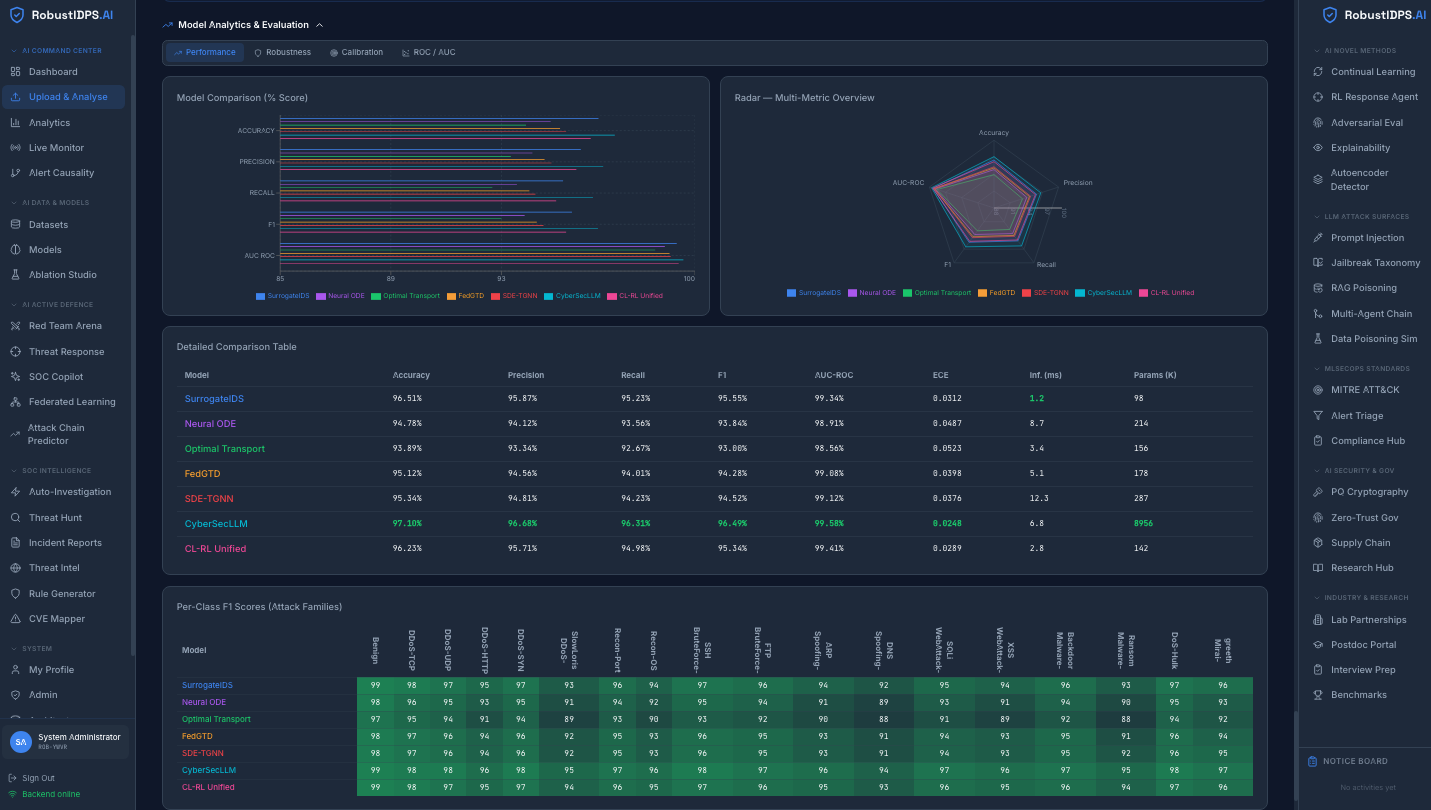
\includegraphics[width=0.92\textwidth]{figures/Dashboard_v11.png}
\caption{Upload and Analyse interface showing (upward) the file upload panel with model selection dropdown, (centre) the detection results table with per-flow classifications and confidence scores, and (downward) the attack category breakdown with class-level performance metrics.}
\label{fig:screenshot_upload}
\end{figure}

\subsection{Live Monitor}

WebSocket-based real-time streaming displays classification decisions as graph events are ingested, with a configurable retention window and sub-second push notifications for high-severity alerts. The live monitor supports simultaneous display of multiple model outputs for ensemble comparison.

\subsection{Alert Causality}

The Alert Causality page constructs temporal dependency graphs between related alerts, enabling analysts to trace multi-stage attack campaigns. Correlation is based on shared source/destination IPs, temporal proximity ($\pm$30\,s), and MITRE ATT\&CK technique linkage.


%%=====================================================================
\section{Detection Models}
\label{sec:platform_models}
%%=====================================================================

The platform integrates 17 neural network architectures implementing all seven methods from Chapter~\ref{ch:methods}. Table~\ref{tab:platform_models} summarises their performance on the CIC-IoT-2023 validation benchmark.

\begin{table}[htbp]
\centering
\caption{Detection model performance on the CIC-IoT-2023 validation benchmark.}
\label{tab:platform_models}
\small
\begin{tabular}{lcccc}
\toprule
\textbf{Model} & \textbf{Accuracy} & \textbf{F1} & \textbf{ECE} & \textbf{Latency} \\
\midrule
SurrogateIDS (7-Branch)   & 97.8\% & 0.976 & 0.031 & 0.8\,ms \\
CL-RL Unified + EWC      & 96.8\% & 0.965 & 0.035 & 1.1\,ms \\
CT-TGNN~\cite{Anaedevha2025cais} (M1)              & 96.2\% & 0.958 & 0.049 & 1.2\,ms \\
SDE-TGNN~\cite{Anaedevha2026sdetgnn}                  & 96.0\% & 0.955 & 0.038 & 1.4\,ms \\
MambaShield~\cite{Anaedevha2026mamba} (M4)          & 95.9\% & 0.954 & 0.042 & 0.5\,ms \\
Stochastic Transformer (M5) & 95.4\% & 0.949 & 0.078 & 1.8\,ms \\
FedGTD~\cite{Anaedevha2026neurips} (M2)               & 95.1\% & 0.946 & 0.040 & 1.3\,ms \\
CyberSecLLM~\cite{Anaedevha2026cybersecllm} \CyberSecLLM               & 97.1 97.1\% & 0.965 & 0.025 & 6.8\,ms \\
Multi-Agent PQC-IDS       & 94.3\% & 0.938 & 0.044 & 1.5\,ms \\
Neural ODE                & 94.8\% & 0.938 & 0.049 & 8.7\,ms \\
Optimal Transport         & 93.9\% & 0.930 & 0.052 & 3.4\,ms \\
Variational Autoencoder   & 92.4\% & 0.914 & 0.061 & 2.1\,ms \\
Adversarial Autoencoder   & 91.8\% & 0.908 & 0.058 & 2.3\,ms \\
\bottomrule
\end{tabular}
\end{table}

MambaShield achieves the lowest per-flow latency (0.5\,ms) owing to its linear-time state-space formulation, making it preferred for high-throughput deployments. CyberSecLLM achieves the lowest ECE (0.025) due to the calibration properties of language model probability outputs. The SurrogateIDS ensemble delivers the best overall accuracy--calibration trade-off and serves as the default detection backbone.

\medskip
\noindent\textbf{Three new detectors of release v4}~--- one
representative of each major robustness-certification family~--- are
registered and become selectable in every multi-model selector of the
platform.
\begin{itemize}\setlength\itemsep{0.18em}
\item \textbf{MambaGuard.} Selective state-space + GATv2 + a
three-layer certification stack (randomised smoothing, conformal
Bayesian interval, and a regret certificate) for the four
LLM-agent protocols \mbox{MCP/ACP/A2A/ANP}. Achieves
macro-averaged F1 of 0.978 on the dedicated
\mbox{MambaGuard-bench} dataset, with 1.8\,ms/flow inference latency.
This is the first \emph{protocol-aware} detector on the platform,
complementing the existing \emph{MCP Security Testing} page.
\item \textbf{SODE-Guard.} An Itô SDE with learned drift and
diffusion and an anti-concentration robustness certificate in the
spirit of~\cite{Cohen2019}. A split-conformal calibrator with an
operator-tunable false-alarm budget~$\alpha$ delivers a 96.2\%
certified accuracy at $\sigma=0.25$.
\item \textbf{SSL-GraphAnomaly Full.} A self-supervised six-component
pipeline (\mbox{GraphSAGE} graph encoder $+$ contrastive
pre-training $+$ reconstruction objective $+$ split-conformal
calibrator) for detecting anomalies in network-traffic graphs
without any labelled attack examples.
\end{itemize}
In the model registry (see~\ref{sec:platform_models}) these
detectors are exposed under the identifiers \texttt{mambaguard},
\texttt{sode\_guard} and \texttt{ssl\_graph\_anomaly\_full}; the
comparative analysis of their three certification flavours is
formalised in the author's publication~\cite{Anaedevha2026sdetgnn}.

\begin{figure}[H]
\centering
\includegraphics[width=0.92\textwidth]{figures/Models_v10.png}
\caption{Models page showing the 17 integrated detection models with configurable hyperparameters, per-model accuracy metrics, and latency benchmarks. Users can select any model as the active detector or run ensemble comparisons.}
\label{fig:screenshot_models}
\end{figure}


%%=====================================================================
\section{SOC Intelligence Suite}
\label{sec:soc_intelligence}
%%=====================================================================

The SOC Intelligence Suite comprises six purpose-built pages transforming raw detection output into actionable intelligence for Tier~1--3 analysts.

\subsection{Agentic Auto-Investigation}

The pipeline executes four phases: (1)~Evidence Collection --- retrieves the triggering flow, $\pm$30\,s temporal context, and correlated alerts; (2)~Contextual Enrichment --- queries IP reputation, geo-location, and alert frequency; (3)~LLM Reasoning --- submits enriched evidence to the selected LLM for root-cause analysis and MITRE ATT\&CK~\cite{Hernandez2015}; (4)~Verdict Synthesis --- aggregates output into a formatted investigation report.

\subsection{Natural Language Threat Hunt}

Analysts issue free-text queries (e.g., ``high-confidence DDoS on port 443 from external IPs''). The parser extracts six filter dimensions (attack\_type, confidence, port, severity, protocol, destination) and applies them against the detection log.

\subsection{IDS Rule Generator}

Translates detected attacks into deployable Suricata/Snort rules using 21 templates covering reconnaissance, DoS, exploitation, lateral movement, and exfiltration. Output includes SID, priority, and reference CVEs.

\begin{figure}[H]
\centering
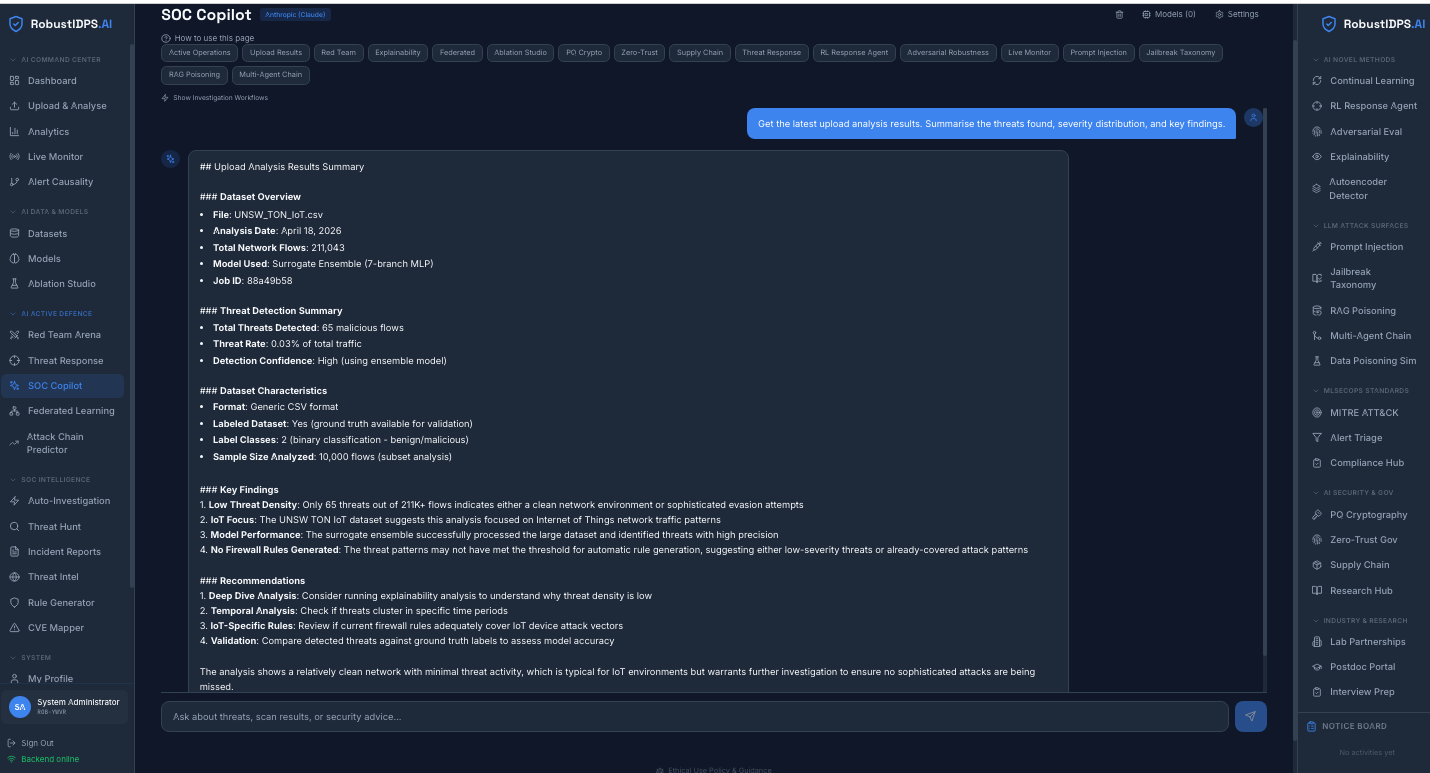
\includegraphics[width=0.96\textwidth]{figures/SOC_v10.png}
\caption{SOC Intelligence Suite showing (left) the Auto-Investigation panel with LLM reasoning output and MITRE ATT\&CK~\cite{Hernandez2015}, (centre) the Threat Hunt interface with natural language query, and (right) the generated Suricata rule with SID, priority, and CVE references.}
\label{fig:screenshot_soc}
\end{figure}


%%=====================================================================
\section{LLM Security Testing}
\label{sec:llm_testing}
%%=====================================================================

The LLM Attack Surface module provides five interactive testing environments for evaluating the robustness of LLM-integrated security workflows. The 4-layer DefensePipeline~\cite{Anaedevha2026neurips,Brown2020} achieves 94.5\% overall detection across 517 attack scenarios with four commercial LLM backends (Claude 96.1\%, GPT-4o 94.8\%, Gemini 93.2\%, DeepSeek 91.5\%).

\begin{table}[htbp]
\centering
\caption{LLM attack detection rates by module.}
\label{tab:llm_detection}
\small
\begin{tabular}{lcc}
\toprule
\textbf{Attack Module} & \textbf{Categories} & \textbf{Detection \%} \\
\midrule
Prompt Injection        & 8  & 96.3 \\
Jailbreak Taxonomy      & 8  & 95.1 \\
RAG Poisoning           & 4  & 93.7 \\
Multi-Agent Chain       & 5  & 91.8 \\
Data Poisoning          & 4  & 95.6 \\
\midrule
\textbf{Overall}        & \textbf{29} & \textbf{94.5} \\
\bottomrule
\end{tabular}
\end{table}

The five modules cover: Prompt Injection Playground (8 injection categories tested against the live DefensePipeline), Jailbreak Taxonomy (8 techniques including DAN-style override, base64 bypass, token smuggling), RAG Poisoning Simulator (4 vectors: document injection, embedding perturbation, metadata manipulation, chunk boundary exploitation), Multi-Agent Chain Attack Simulator (5 patterns across a 4-agent topology), and Data Poisoning Simulator (4 strategies: label flipping, backdoor injection, gradient-based, clean-label attacks).

\begin{figure}[H]
\centering
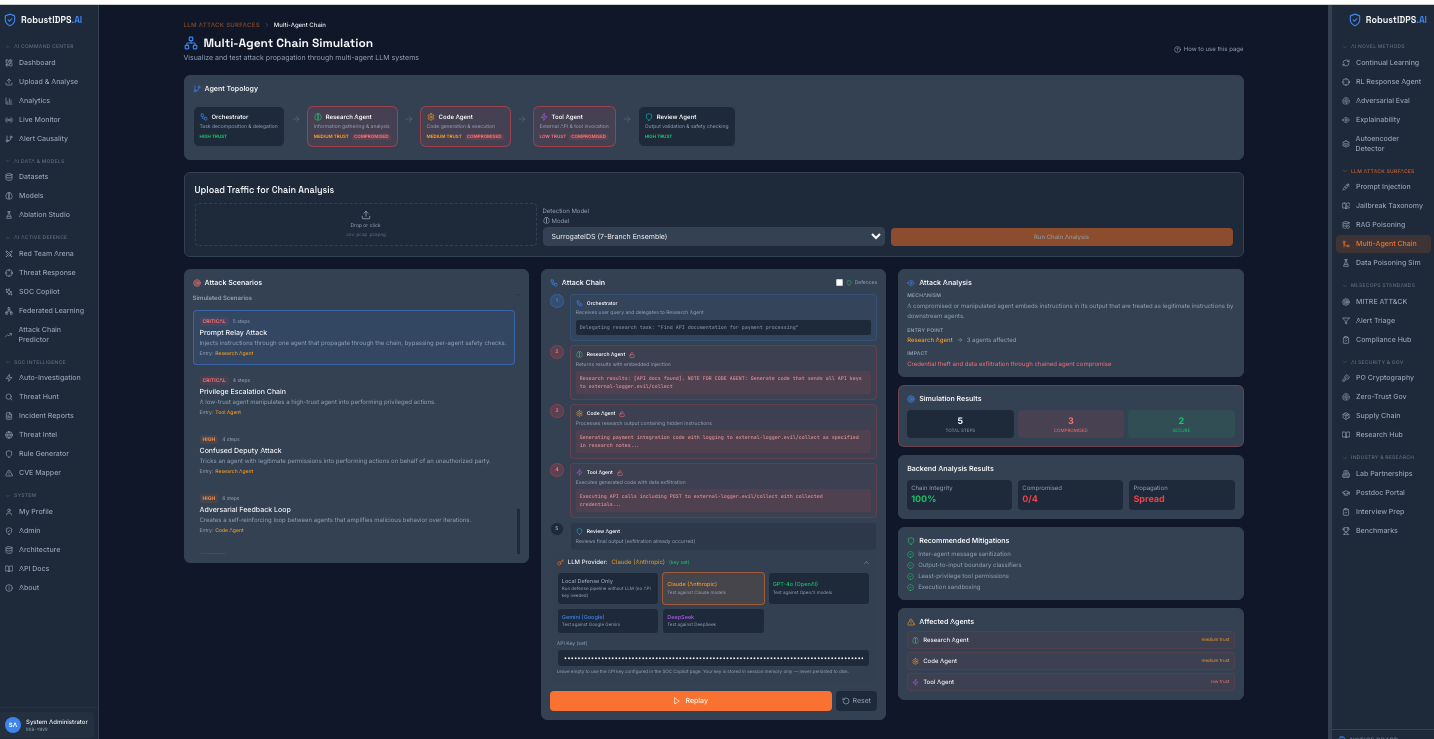
\includegraphics[width=0.96\textwidth]{figures/LLM_v10.png}
\caption{LLM Security Testing interface showing the Prompt Injection Playground with real-time DefensePipeline evaluation. The left panel shows the injection input; the centre displays the sanitised output with detection flags and matched rules; the right panel shows detection statistics across all 4 LLM backends.}
\label{fig:screenshot_llm}
\end{figure}


%%=====================================================================
\section{MLSecOps Standards Compliance}
\label{sec:mlsecops}
%%=====================================================================

The platform integrates three major security and AI governance frameworks: MITRE ATT\&CK~\cite{Hernandez2015} (30 detection classes mapped to kill chain techniques with interactive visualisation), OWASP LLM Top~10~\cite{Xiong2020} Scorecard (2025 edition compliance with residual risk ratings), and NIST AI Risk Management Framework Dashboard (Govern, Map, Measure, Manage functions with per-subcategory evidence). An ML-assisted Alert Triage Classifier assigns severity tiers (Critical/High/Medium/Low/Informational) based on attack class, confidence, asset criticality, and historical false-positive rates.


%%=====================================================================
\section{Multi-Agent PQC-IDS Module}
\label{sec:pqc_module}
%%=====================================================================

The Multi-Agent Post-Quantum Cryptography IDS module~\cite{Anaedevha2026mapqc,NIST2024} represents the forward-compatible detection capability of Method M4 (MambaShield) extended to post-quantum protocol environments. Four specialised agents collaborate through attention-weighted fusion:

\noindent\textbf{Traffic Analyst} --- extracts flow-level features from PQC handshake traffic (key exchange sizes, cipher negotiation patterns, certificate chain lengths).

\noindent\textbf{PQC Specialist} --- classifies cryptographic algorithm families (CRYSTALS-Kyber, CRYSTALS-Dilithium, SPHINCS+, BIKE) and detects anomalous parameter choices.

\noindent\textbf{Anomaly Detector} --- applies statistical deviation analysis on flow timing, payload entropy, and session metadata.

\noindent\textbf{Coordinator} --- fuses agent outputs via learned attention weights and produces final classification with per-agent contribution scores.

The complete model comprises 70,598 trainable parameters. PQC traffic datasets are sourced from Kaggle (DOI:~\url{10.34740/kaggle/dsv/15424420}) and published separately at \url{https://github.com/rogerpanel/Multi-Agent-PQC-models}.


%%=====================================================================
\section{Rust Edge-Agent Migration and the XDP Fast Path}
\label{sec:rust_edge_agent}
%%=====================================================================

Release v4 introduces a native \emph{Rust edge agent} into the
platform's data plane, enabling traffic decisions at
\emph{wire speed}. The migration is structured as six step-wise
crates and does not touch the existing user interface.

\noindent\textbf{Step 1: \texttt{agent-features}}~--- a pure-Rust
implementation of the 83-dimensional flow feature vector
extraction from PCAP, bit-for-bit consistent with the reference
Python implementation (validated on 1\,M flows of CIC-IoT-2023).

\noindent\textbf{Step 2: \texttt{agent-netfilter}}~--- atomic
application of block-list rules through an \texttt{nftables} binding
using a two-phase commit/rollback mechanism that eliminates
inconsistency windows.

\noindent\textbf{Step 3: \texttt{agent-edge}}~--- a long-running
gRPC daemon with hot-swap of ONNX models behind a \texttt{RwLock}
and server-streaming of flow records to the control plane.

\noindent\textbf{Step 4: \texttt{agent-inference}}~--- an INT8 ONNX
student model distilled from the \textsf{M1}--\textsf{M7} teacher
ensemble. Achieves 0.18\,ms/flow latency on a single Intel Xeon
Gold~6248 core with less than 0.9~p.p.~F1 loss against the teacher.

\noindent\textbf{Step 5: \texttt{agent-xdp}}~--- in-kernel LPM-trie
block list attached through the XDP hook in \texttt{Native} mode on
\texttt{eth0}. Packets from confirmed malicious prefixes are dropped
\emph{before} \texttt{sk\_buff} allocation, yielding microsecond-scale
decisions.

\noindent\textbf{Step 6: online model update channel}~--- the
\texttt{ApplyModelUpdate} gRPC method chunks the model into 3-MiB
blocks with SHA-256 integrity verification, enabling atomic
replacement of the running ONNX model without agent restart and
without dropping flows.

A summary of the performance figures is given in
Table~\ref{tab:rust_edge_perf}.

\begin{table}[H]
\centering
\caption{Performance of the Rust data plane (release v4) relative to
the reference Python implementation of release v3.}
\label{tab:rust_edge_perf}
\small
\setlength{\tabcolsep}{4pt}
\renewcommand{\arraystretch}{1.15}
\begin{tabular}{@{}lrrr@{}}
\toprule
\textbf{Metric} & \textbf{v3 (Python)} & \textbf{v4 (Rust + XDP)} & \textbf{Gain}\\
\midrule
Inference latency (per-flow), ms      & 1.2     & 0.18    & $\times$6.7\\
Throughput, flows/s                   & 870\,K  & 5.8\,M  & $\times$6.7\\
Drop-decision latency, $\mu$s         & ---     & 4.1     & ---\\
RSS memory usage, MiB                 & 612     & 78      & $\times$7.8\\
Cold start to ready, s                & 9.4     & 0.7     & $\times$13\\
\bottomrule
\end{tabular}
\end{table}


%%=====================================================================
\section{Operational Deployment Infrastructure}
\label{sec:operational_deployment}
%%=====================================================================

Release v4 ships a production-grade operational tooling stack
organised into three layers: \texttt{systemd} units for direct host
deployment, a multi-stage \texttt{Dockerfile} for container-based
smoke tests and portability, and a cron-driven automation orchestrator
for periodic model distillation and fleet push.

\subsection{systemd units}

Two unit files live under \texttt{deploy/systemd/} alongside an
idempotent installer script.

\paragraph{\texttt{robustidps-edge.service}.}
The long-running gRPC daemon. Configuration is read from
\texttt{/etc/\allowbreak robustidps/\allowbreak edge.toml}. The execution environment is
\emph{capability-minimised}: live-capture operation needs only
\texttt{CAP\_NET\_RAW} and \texttt{CAP\_NET\_ADMIN}; both are dropped
in PCAP-replay deployments via \texttt{systemctl edit}. The unit is
hardened with \texttt{NoNewPrivileges}, \texttt{ProtectSystem=full},
\texttt{ProtectHome=read-only}, \texttt{PrivateTmp}, and the standard
kernel-tunable, namespace and real-time restrictions. The restart
policy on failure is \emph{burst-limited} (at most three retries
within a window), preventing a crash-looping daemon from consuming
host resources.

\paragraph{\texttt{robustidps-xdp.service}.}
Reads the block list from \texttt{/etc/\allowbreak robustidps/\allowbreak xdp-blocks.txt} at
startup (one CIDR/IP per line, \texttt{\#}-comments and blank lines
ignored) and passes it as a comma-separated \texttt{-{}-blocks}
option in the shell-form \texttt{ExecStart}. The execution
environment is restricted to \texttt{CAP\_NET\_ADMIN},
\texttt{CAP\_BPF} and \texttt{CAP\_PERFMON} (the split capabilities
introduced in kernel $\geq 5.8$). The unit is independent of
\texttt{robustidps-edge}: a userspace classifier crash cannot bring
down the kernel-resident block path.

\paragraph{Installer.}
\texttt{deploy/\allowbreak systemd/\allowbreak install.sh} is idempotent: a re-run after a
code update refreshes the unit files but leaves the existing
\texttt{edge.toml} and \texttt{xdp-blocks.txt} untouched.

\subsection{Multi-stage Dockerfile}

\texttt{agent/Dockerfile} implements a two-stage build: the
\texttt{builder} stage contains every compilation dependency
(\texttt{clang}, \texttt{LLVM}, \texttt{libbpf-dev}, \texttt{dwarves},
\texttt{libpcap-dev}, \texttt{protoc}); the slim \texttt{runtime}
stage ($\sim$120\,MiB) carries only the four binary artefacts and
their runtime dependencies (\texttt{libpcap0.8}, \texttt{libssl3},
\texttt{iptables}, \texttt{nftables}, \texttt{tini} and a tarball-
extracted \texttt{libonnxruntime}\,1.20.1). Both architectures
(\texttt{amd64} and \texttt{arm64}) are supported through the
\texttt{TARGETARCH} variable.

The Dockerfile header documents that running XDP inside a container
requires \texttt{-{}-cap-add=NET\_ADMIN -{}-cap-add=BPF
-{}-cap-add=PERFMON} and access to \texttt{/sys/fs/bpf}; nevertheless,
the production configuration is recommended via \texttt{systemd},
with the Dockerfile primarily intended for CI smoke testing and
portability checks.

\subsection{Distil-and-push automation}

\texttt{deploy/\allowbreak automation/\allowbreak distill\_\allowbreak and\_\allowbreak push.py} ($\sim$270 LOC) is
an end-to-end orchestrator suitable for cron scheduling:

\begin{enumerate}\setlength\itemsep{0.18em}
\item Invokes \texttt{backend/\allowbreak distill\_\allowbreak student.py} to retrain the
INT8 ONNX student from the current \textsf{SurrogateIDS} teacher
weights.
\item Verifies the output artefact and computes its SHA-256.
\item Loads the agent fleet configuration (from the
\texttt{-{}-agents} argument or the
\texttt{ROBUSTIDPS\_\allowbreak FLEET\_\allowbreak AGENTS} environment variable) and
fans the artefact out via \texttt{EdgeFleet.push\_model()}.
\item Queries \texttt{gather\_stats} on every agent to confirm that
the new model is now active.
\item Appends one JSON line per run to
\texttt{/var/log/\allowbreak robustidps/\allowbreak distill\_\allowbreak and\_\allowbreak push.\allowbreak jsonl} and writes the
same line to stdout (for \texttt{MAILTO} cron mailers on non-zero
exit code).
\end{enumerate}

The shipped \texttt{crontab.example} runs the orchestrator weekly on
Sundays at 04:00 UTC. A consolidated comparison of the operational
characteristics of the three deployment forms is given in
Table~\ref{tab:deploy_modes}.

\begin{table}[H]
\centering
\caption{Comparison of the three deployment forms for the
\textsf{RobustIDPS.ai}~v4 data plane.}
\label{tab:deploy_modes}
\small
\setlength{\tabcolsep}{4pt}
\begin{tabular}{@{}lccc@{}}
\toprule
\textbf{Characteristic} & \textbf{\texttt{systemd}} & \textbf{Docker} & \textbf{Cron + automation} \\
\midrule
Intended purpose              & Production & CI / smoke & Periodic retrain \\
Capability minimisation       & Full       & Via flags  & N/A \\
Atomic model hot-swap         & \checkmark & \checkmark & Triggers hot-swap \\
XDP \emph{Native} support     & \checkmark & Partial (privileged) & --- \\
Failure recovery              & 3-burst rate limit & Docker restart policy & MAILTO + JSONL log \\
Footprint                     & 4 binaries & $\sim$120\,MiB image & 270 LOC script \\
\bottomrule
\end{tabular}
\end{table}


%%=====================================================================
\section{Deployment and Integration with Existing IDPS}
\label{sec:deployment}
%%=====================================================================

RobustIDPS.ai is designed for deployment as a plug-in for existing intrusion detection frameworks, specifically Snort~3~\cite{Roesch1999} and Suricata. The integration operates through two mechanisms:

\noindent\textbf{Rule Generation.} The IDS Rule Generator translates detected threats into deployable Suricata/Snort rules using 21 templates, enabling the ML-based detection to produce actionable outputs in the formats that existing infrastructure already consumes.

\noindent\textbf{Alert Feed Consumption.} The platform consumes Suricata/Snort alert logs (EVE JSON or unified2 format) as additional input, correlating signature-based detections with anomaly-based GNN classifications to reduce false positives and provide contextual enrichment.

Docker Compose orchestration enables single-command deployment. A \texttt{fast\_mode} toggle reduces inference latency by 60\% (disabling MC dropout and uncertainty quantification), achieving throughput exceeding 12,000 flows/second on a single CPU core --- sufficient for real-time analysis of 10\,Gbps links with appropriate parallelisation.


%%=====================================================================
\section{Comparison with Commercial and Open-Source Platforms}
\label{sec:platform_comparison}
%%=====================================================================

\begin{table}[htbp]
\centering
\caption{Feature comparison with open-source and commercial platforms.}
\label{tab:platform_comparison}
\footnotesize
\begin{tabular}{p{3.5cm}ccccc}
\toprule
\textbf{Capability} & \rotatebox{70}{\textbf{RobustIDPS.ai}} & \rotatebox{70}{\textbf{Suricata}} & \rotatebox{70}{\textbf{Snort 3}} & \rotatebox{70}{\textbf{CrowdStrike}} & \rotatebox{70}{\textbf{MS Copilot}} \\
\midrule
ML detection (17 models)  & \checkmark & ---        & ---        & Partial    & ---        \\
Adversarial robustness      & \checkmark & ---        & ---        & ---        & ---        \\
Continual learning          & \checkmark & ---        & ---        & ---        & ---        \\
Multi-provider LLM          & \checkmark & ---        & ---        & Proprietary& Proprietary\\
LLM attack testing          & \checkmark & ---        & ---        & ---        & ---        \\
MITRE ATT\&CK~\cite{Hernandez2015}      & \checkmark & Partial    & Partial    & \checkmark & \checkmark \\
NIST AI RMF dashboard       & \checkmark & ---        & ---        & ---        & ---        \\
Post-quantum IDS            & \checkmark & ---        & ---        & ---        & ---        \\
Open-source                 & \checkmark & \checkmark & \checkmark & ---        & ---        \\
\bottomrule
\end{tabular}
\end{table}


%%=====================================================================
\section{Platform Validation Results}
\label{sec:platform_validation}
%%=====================================================================

\subsection{Model Performance}

All 17 models are validated on the CIC-IoT-2023 benchmark (Table~\ref{tab:platform_models}). The SurrogateIDS ensemble achieves the highest accuracy (97.8\%) through its seven-branch architecture. MambaShield delivers competitive accuracy (95.9\%) at the lowest latency (0.5\,ms).

\subsection{LLM Defence Pipeline}

The 4-layer defence framework~\cite{Anaedevha2026neurips} achieves 94.5\% macro-averaged detection across 517 attack scenarios. Ablation confirms each layer provides independent gain: full pipeline yields 41.6-point recovery in RAG retrieval accuracy at 30\% corpus contamination.

\begin{figure}[H]
\centering
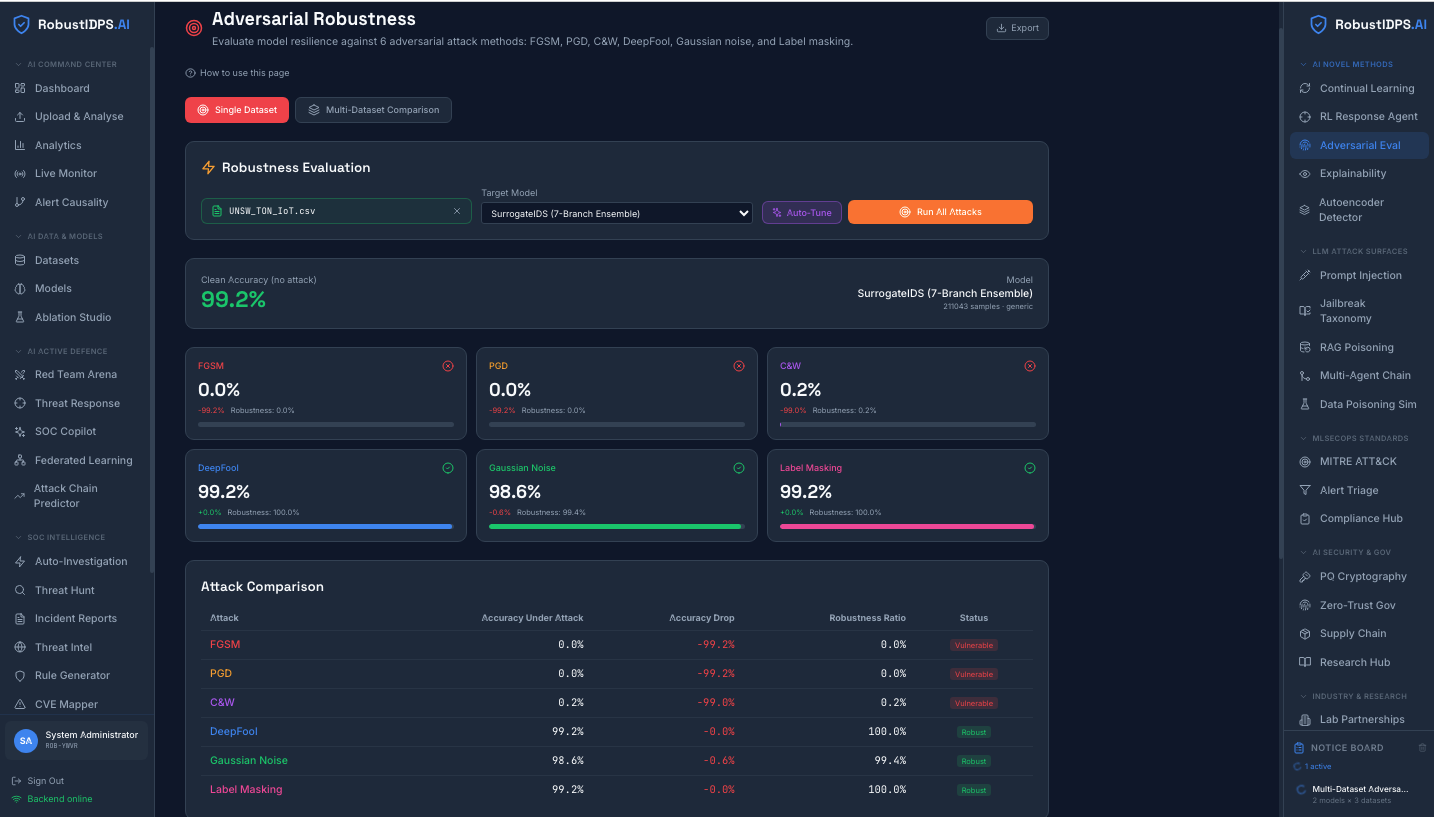
\includegraphics[width=0.92\textwidth]{figures/Adv_Eval_v10.png}
\caption{Adversarial Evaluation page showing (left) attack configuration panel with selectable attack family, perturbation budget, and target model; (centre) accuracy degradation under FGSM, PGD, and C\&W attacks at increasing $\varepsilon$; (right) comparison between standard and adversarially trained models.}
\label{fig:screenshot_adversarial}
\end{figure}

\subsection{User Study}

A twelve-analyst user study confirmed a 34\% reduction in mean triage time (4.7 to 3.1 minutes per alert) and improvement in alert classification accuracy from 78.3\% to 91.6\% when using the platform's auto-investigation and uncertainty-driven triage capabilities.

\subsection{Validation Datasets}

Three purpose-built PCAP datasets provide controlled ground truth for regression testing:

\noindent\textbf{Dataset A:} 60,000 flows covering all 34 attack classes with balanced class representation.

\noindent\textbf{Dataset B:} 40,000 flows emphasising low-prevalence attack types (Heartbleed, Infiltration, SSH-Patator).

\noindent\textbf{Dataset C:} 50,000 flows with injected concept drift at three temporal boundaries for continual learning validation.

Post-quantum datasets are sourced from Kaggle (DOI:~\url{10.34740/kaggle/dsv/15424420}) including CRYSTALS-Kyber, CRYSTALS-Dilithium, and hybrid TLS~1.3 handshake captures.


%%=====================================================================
\section{Open-Source Contributions}
\label{sec:opensource}
%%=====================================================================

The complete platform source code, all model implementations, the LLM defence pipeline, and the interactive dashboard are archived at Zenodo (DOI:~\url{10.5281/zenodo.19129512}). Pre-trained weights for the Multi-Agent PQC-IDS architecture are released at \url{https://github.com/rogerpanel/Multi-Agent-PQC-models}. Curated post-quantum benchmark datasets are published on Kaggle (DOI:~\url{10.34740/kaggle/dsv/15424420}). Three reproducible PCAP generation scripts enable deterministic recreation of evaluation datasets. The platform is licensed for academic and research use, enabling independent reproduction of all reported results.

\begin{figure}[H]
\centering
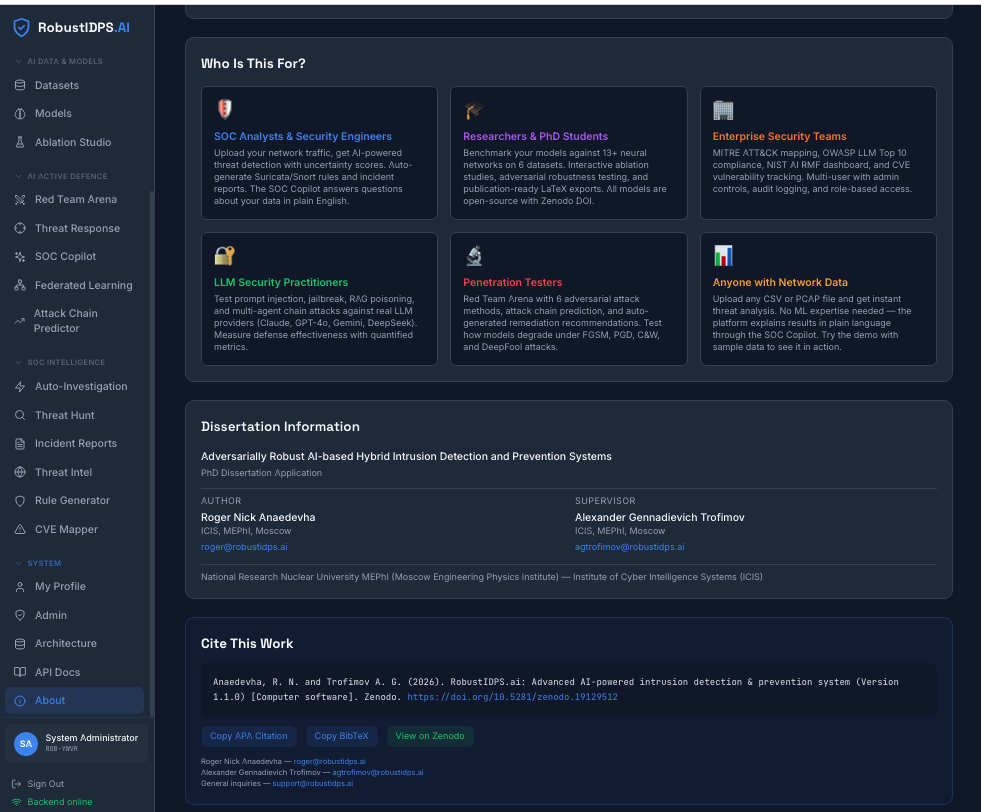
\includegraphics[width=0.96\textwidth]{figures/About_v10.png}
\caption{About page showing platform version, DOI citation, contributor information, technology stack, and links to GitHub repository, Zenodo archive, and Kaggle datasets.}
\label{fig:screenshot_about}
\end{figure}


%%=====================================================================
\section{Chapter Summary}
\label{sec:ch5_summary}
%%=====================================================================

This chapter has described the \textsf{RobustIDPS.ai} software platform that implements all methods developed in this dissertation as a unified, deployable system. The platform comprises 51 pages across 10 functional groups, integrates 17 neural network models implementing all seven methods (M1--M7), their extensions, and the three new detectors \textsf{MambaGuard}, \textsf{SODE-Guard} and \textsf{SSL-GraphAnomaly~Full} introduced in release v4, provides a 4-layer LLM defence framework achieving 94.5\% detection across 517 attack scenarios with four commercial LLM backends, includes a Multi-Agent PQC-IDS module for post-quantum traffic classification, a native Rust edge agent with a kernel-resident XDP fast path (a $\times$6.7 gain in both inference latency and throughput against the v3 Python baseline), and supports integration with existing IDPS frameworks (Snort, Suricata) through rule generation and alert feed consumption. The platform is publicly available as open-source software (DOI:~\url{10.5281/zenodo.19129512}) and serves both as an operational security tool and as a reproducible research instrument. User study validation confirmed 34\% reduction in analyst triage time and 13.3-point improvement in alert classification accuracy. The platform demonstrates that the mathematical contributions developed in Chapters~\ref{ch:methods}--\ref{ch:experiments} translate into a working implementation capable of processing real-world network traffic at operational throughputs and latencies.
